\documentclass[a4paper]{report}
\usepackage[14pt]{extsizes}
\usepackage[utf8]{inputenc}
%\usepackage[T1]{fontenc}
\usepackage[french]{babel}
\usepackage{makeidx}
\usepackage{graphicx}
\usepackage{listingsutf8}
\usepackage{verbatim}
\usepackage{calc}
\usepackage{tikz}
\usepackage{titlesec} 
\usepackage{hyperref}
\hypersetup{
    colorlinks,
    citecolor=black,
    filecolor=black,
    linkcolor=black,
    urlcolor=black
}
\title{RAPPORT DU PROJET STL \\ TIKZ}
\author{ANCELIN Maxime & DIAKHATE Aminata}

\lstset{language=Perl}
\lstset{commentstyle=\textit}
\lstset{frame=shadowbox, rulesepcolor=\color{gray}}

\begin{document} 

\newenvironment{violetpar}{\color{violet}}{}
\newenvironment{bluepar}{\par\color{blue}}{\par}
\newenvironment{yellowpar}{\par\color{orange}}{\par}

\renewcommand{\labelitemi}{$\bullet$}

\setcounter{tocdepth}{3}
%\makeatletter
%\newcounter {subsubsubsection}[subsubsection]
%\renewcommand\thesubsubsubsection{\thesubsubsection .\@alph\c@subsubsubsection}
%\newcommand\subsubsubsection{\@startsection{subsubsubsection}{4}{\z@}%
%                                     {-3.25ex\@plus -1ex \@minus -.2ex}%
%                                     {1.5ex \@plus .2ex}%
%                                     {\normalfont\normalsize\bfseries}}
%\newcommand*\l@subsubsubsection{\@dottedtocline{3}{10.0em}{4.1em}}
%\newcommand*{\subsubsubsectionmark}[1]{}
%\makeatother

\maketitle
\tableofcontents
\newpage

\titleformat{\chapter}[hang]{\bf\huge}{\thechapter}{2pc}{} 


\newpage
 \chapter{Introduction}
  Dans le cadre de notre enseignement universitaire à l'UPMC(Université Pierre Marie Curie) en master Science et Technologie du Logiciel, nous devons réaliser un projet proposé par nos professeurs. C'est ainsi que nous avons choisi le sujet proposé par Monsieur Frederic Peschanski qui est de créer une interface graphique au dessus d'un sous-ensemble du langage Tikz, permettant la construction visuelle (plutôt que textuelle) des figures. 
  \newline
  Nous allons tout au long de notre rapport vous expliquer comment nous avons gérer ce projet. Nous commencerons donc par vous faire une présentation générale de notre projet. Ensuite, nous vous parlerons de la gestion de notre projet ; et pour finir nous vous présenterons nos perspectives pour ce projet.
  
  \chapter{Présentation du projet}
  \section{Contexte}
  LaTex(Lamport TEX) est un langage et un système de composition de documents. Du fait de sa relative simplicité, il est souvent utilisé dans les domaines techniques et scientifiques pour la production d'un contenu complexe (équations, graphes, ...) ayant une mise en forme standard. Afin d'inclure ces contenus complexes dans les documents en restant dans l'environnement LaTex, LaTex dispose d'un package TikZ permettant d'inclure des figures au format PDF. En effet, TikZ permet d'obtenir des figures géométriques complexes précise et d'une grande qualité. Cependant son apprentissage n'est pas évident. 
  \subsection{Motivations}
  Notre encadrant, qui est lui-même un utilisateur de TikZ, a souhaité faciliter l'utilisation de TikZ afin de permettre à un plus grand nombre d'utilisateurs de profiter de ses avantages sans forcément passer par son apprentissage. Pour ce faire, il nous propose donc de mettre en place une interface graphique permettant la construction  visuelle (et non textuelle) des figures.
  \newline
  Pour ce projet que nous devions réaliser dans le cadre de notre master, nous avions souhaité, avant même de 
connaître les sujets proposés, de choisir un projet qui nous permettrait de nous rapprocher le plus de ceux qu'on pourrait rencontrer dans le monde professionnel. Par la suite après avoir étudié tous les sujets proposés, ce projet a retenu notre attention parce qu'il nous permettait d'approfondir nos connaissances tout en réalisant un projet qui diffère de nos projets habituels.
  \section{Objectifs}
  Notre objectif est de pouvoir présenter au terme de ce projet une interface graphique qui permettrait à l'utilisateur de pouvoir créer des graphes non plus textuellement mais visuellement. L'interface graphique devra aussi permettre à l'utilisateur de rédiger du code TikZ et visualiser le graphe correspondant ou encore modifier le graphe en bougeant les noeuds sélectionnés ou en modifiant leurs propriétés grâce à un menu.
Toute modification apportée au graphe devra mettre à jour le code source correspondant et vice-versa. 
  \chapter {Gestion du projet}

  \section{Choix technologiques}
  Pour la réalisation de notre projet, notre encadrant nous a recommandé l'utilisation d'un langage de script tel que Python ou Ruby, permettant l'interfaçage avec des outils externes (notamment pdflatex avec le paquet "preview") et les manipulations textuelles simples (expressions rationnelles etc.), et proposant de plus des bibliothèques portables pour les interfaces utilisateurs (Gtk, Qt, WxWindows, etc.). Même si notre encadrant nous a vivement conseillé l'utilisation de Python nous avons quand même choisi de faire notre projet avec Perl. 

Perl nous a semblé être un bon choix de langage car il est adapté au traitement et manipulation de fichiers texte du fait de l'intégration des expressions régulières dans la syntaxe même du langage or nous voulions manipuler des fichers LaTex et Tikz; de plus perl est portable sur la plupart des systèmes d'exploitation, il devient même populaire sous Windows grâce à la distribution gratuite ActivePerl. 
Pour l'interface utilisateur nous avons choisi la bibliothèque Qt comme nous le conseillait notre encadrant. Au final nous avons donc utiliser PerlQt qui allie la souplesse, la puissance et le design élégant de Qt au langage Perl. Pour l'installater, nous avons dû choisir entre deux versions de PerlQt4:
\begin{itemize}
 \item Une version avec une vue sur Qt-sys.org publié par l'utilisateur "vadiml" et qui n'a pas été mise à jour depuis Février 2008
 \item Une autre avec une vue sur code.google.com publié par "chrisburel@gmail" qui semblait plus complète et surtout activement maintenue puisque la dernière version datait de quelques jours seulement(février 2012).
\end{itemize}
  Notre choix c'est donc naturellement porté sur la version proposée par "chrisburel@gmail".
  \newline 
  Pour notre interface graphique, nous avions besoin d'un éditeur qui nous permettrait d'écrire du code Tikz. Pour cela nous avons choisi Scintilla qui est un composant d'édition de code open source. En effet Scintilla a beaucoup de fonctionnalités qui rendent l'édition de code plus facile telles que la coloration syntaxique, la gestion des numéros de ligne dans la marge, les points d'arrêts pour le débogueur, etc.
  \newline
  Au début de notre projet nous n'avions pas utiliser de gestionnaire de version car nous travaillions le plus souvent ensemble. D'ailleurs à la première semaine de notre projet nous avions réaliser le mokup de notre interface avec Michael MENU, un étudiant de notre promotion qui avait le même sujet que nous mais développé en Python. Pendant les vacances scolaires du mois d'avril où la distance ne nous permettait pas de continuer à travailler ensemble, nous avons installé git qui est un logiciel de gestion de versions décentralisé libre. 
  
\chapter {Gestion du projet}
\section{Difficultés}
\subsection{Installation de perlqt4}
L' installation de perlqt4 nous a pris un peu plus d' une semaine,
car il nous manquait des dépendances.

Au fur et à mesure que nous découvrions ce qu' il fallait ajouter,
nous avons enrichi un script d' installation afin de rendre la réinstallation
plus facile pour les utilisateurs finaux de notre application. Ce
script a été conçu pour fonctionner sous \textit{Ubuntu 12.04} et devrait marcher
sans encombre sous \textit{Debian}.

Sous ces \textit{linux}, il suffit de lancer \textbf{script\_intall\_all.sh}
afin d' installer \textit{perlqt4}, \textit{Scintilla} et tout les packages et modules
\textit{Perl} requis au fonctionnement de l' application.

\subsection{Génération d'une image png à partir d'un code Tikz}
Notre éditeur de texte sur \textbf{TikzG} ne contient que le code d'une figure Tikz, c'est à dire les instructions comprises entre \verb?\begin[tikzpicture]? et \verb?\end[tikzpicture]?. Ce code n'est pas directement compilable.

Afin de générer un pdf valide en fonction du code Tikz et d'ajuster la taille du pdf a celle de la figure Tikz, nous encapsulons le \textcolor{blue}{code} entre un \textcolor{violet}{préambule} \textit{latex/tikz} et un \textcolor{orange}{postambule} \textit{tikz/latex} et sauvegardons le tout dans un fichier tex temporaire : \textit{tmp\_tikz.tex}.

\newpage

\hrule
\begin{violetpar}
\begin{verbatim}
\documentclass{article}
\usepackage[graphics,tightpage,active]{preview}
\usepackage[utf8]{inputenc}  
\usepackage{xcolor}
\usepackage{tikz}
\PreviewEnvironment{tikzpicture}
\begin{document}
\begin{tikzpicture}\end{verbatim}
\end{violetpar}
\begin{bluepar}
\begin{verbatim}[node distance=40pt]
\node[rectangle,draw] (n1) {a};
\node[circle,double,draw,right of=n1] (n2) {$\sqrt{x}$};
\draw[->] (n1) -- (n2);
\node[below of=n1,right of = n1,node distance=50pt] (n3) {c};
\draw[<->,dashed] (n1) -- (n3);
\end{verbatim}
\end{bluepar}
\begin{yellowpar}
\begin{verbatim}
\end{tikzpicture}
\end{document}
\end{verbatim}
\end{yellowpar}
\hrule
\begin{flushright}
tmp\_tikz.tex
\end{flushright}

Le fichier tex ainsi assemblé est ensuite compilé a l'aide de la commande pdflatex, créant le fichier \textit{tmp\_latex.pdf}. Afin de ne pas bloquer notre application si la compilation du fichier tex échoue, on utilise l'option \textit{-halt-on-error} de pdflatex.
Pour accélerer la génération du pdf, on supprime l'affichage des messages de compilations de pdflatex en redirigeant la commande vers \textbf{/dev/null}
\begin{lstlisting}[language=bash]
pdflatex -halt-on-error tmp_tikz.tex > /dev/null
\end{lstlisting}
Ce fichier pdf est ensuite converti en png à l'aide de la commande \textbf{convert} du logiciel libre \textit{ImageMagick}, puis affichée dans un composant flottant de la fen\^etre principale.
La fonction de génération d'image par rapport au code Tikz peut être appellée :
\begin{itemize}
\item Manuellement (en cliquant \textit{Génerer image} ou en faisant le racourci Ctrl+R)
\item Automatiquement (Si le code Tikz courrant n' a pas deja été généré, 1 seconde d'innaction depuis la derniére modification du code de l'éditeur Tikz)
\end{itemize}
\subsection{Modifier l'échelle d'une image générée}
A partir du pdf généré par \textbf{pdflatex}, nous pouvons connaitre la taille finale de l'image.
Le paramétre \textbf{density} de la commande \textbf{convert} permet de jouer sur l'échelle de l'image sans perdre de qualité.
À l'aide d'un script, nous avons transformé un même pdf en plusieurs png de résolutions différentes.
\newline
\\
\parbox{1.15\textwidth}{
{\small \lstinputlisting[inputencoding=utf8/latin1]{script_density.pl}}
}
En regardant la taille des des images produites, nous avons pu déduire que :
\begin{itemize}
\item Pour une valeur de \textbf{density} de \textbf{72}, l'échelle de l'image est de \textbf{100\%}
\item L'échelle de l'image est \textbf{int((density/18) * 25)}
\end{itemize}


\subsection{Analyse des logs pdflatex}
Si le code Tikz est incorrect, la commande pdflatex sera interompue et aucun pdf valide ne sera produit.
Les fichiers de logs de latex sont trés longs et verbeux (par exemple, pour une figure tikz d' une dizaine de lignes, nous avons 574 lignes de logs). Pour aller à l'essentiel des messages d'erreurs et afficher la ligne d'erreur en fonction de notre éditeur, nous avons mis en place un parseur. L'affichage des messages se fait si besoin dans notre fenêtre principale.

Ce parseur reconnait de nombreux messages de d'erreurs et a un mécanisme en place pour afficher les messages qui tiennent sur deux lignes. Il doit être testé avec de nombreux programmes erronés afin de s'assurer qu'il gére bien tous les messages d'erreurs.


\parbox[t]{1.2\textwidth}{
{\small \lstinputlisting[inputencoding=utf8/latin1]{parseur_logs.pl}}
}

\subsection{Creation d'une structure objet pour toute instruction Tikz}
Afin de faciliter l'accés a tous les champs des instructions Tikz composant une figure et de permettre une intéraction avec l'utilisateur, nous avons mis en place une structure objet Tikz.

Cette structure est définie dans le module \textit{TikzObjects.pm}.

Notre programme a une liste interne contenant la liste des instruction de la figure Tikz courante.
Cette liste est crée a chaque génération de l'image png correspondant au code Tikz a l'aide du module \textit{TikzParser.pm}. Nous n'entrerons pas dans les détails de comment sont reconnues et traitées les instructions Tikz par le parseur.
Par la suite, nous allons montrer les champs des différents élèments reconnus par notre parseur d'objets Tikz en montrant un exemple pour chaque type d'instruction.

\subsubsection{nodeDistance}
Cet objet Tikz contient la distance par défault entre deux n{\oe}uds pour la figure Tikz en cours.
\begin{verbatim}
 'ligne' => 1,
 'nodeDistance' => '50pt',
 'type' => 'NodeDistance',
 'code' => '[node distance=50pt]'
\end{verbatim}

\subsubsection{node}
Cet objet Tikz contient tout les champs nécessaires d'un n{\oe}ud.
\begin{verbatim}
 'nom' => 'n2',
 'params_keys' => [
                    'circle',
                    'double',
                    'draw',
                    'right of'
                  ],
 'params' => {
               'double' => undef,
               'right of' => 'n1',
               'draw' => undef,
               'circle' => undef
             },
 'ligne' => 3,
 'text' => '$\\frac{\\sqrt{x}}{x^y}$',
 'type' => 'node',
 'colorId' => 'red!30!green!31,fill=red!30!green!31',
 'code' => '\\node[circle,double,draw,right of=n1] (n2) {$\\frac{\\sqrt{x}}{x^y}$};'
\end{verbatim}

\subsubsection{draw}
Cet objet Tikz contient tout les champs nécessaires d'une ar\^ete.
\begin{verbatim}
 'ligne' => 4,
 'colorId' => 'red!30!green!32,fill=red!30!green!32',
 'params' => {
               '->' => undef
             },
 'params_keys' => [
                     '->'
                  ],
 'origine' => 'n1',
 'type' => 'draw',
 'but' => 'n2',
 'code' => '\\draw[->] (n1) -- (n2);',
 'code_segment' => ' -- '
\end{verbatim}

\subsubsection{NoCode}
Cet objet Tikz contient une ligne vide, sans instruction.
\begin{verbatim}
 'ligne' => 13,
 'type' => 'NoCode',
 'code' => ''
\end{verbatim}

\subsubsection{unknown}
Cet objet Tikz contient toute instructions Tikz non reconnue par notre parseur (ni \textit{node}, ni \textit{draw}).
\begin{verbatim}
 'ligne' => 2,
 'type' => 'unknown',
 'code' => 
   '\\tikz \\foreach \\r in {1,2,...,5} \\draw (0,0) circle (\\r mm);'
\end{verbatim}

\subsection{Identification des objets Tikz}
Afin d' identifier précisément chaque objet Tikz, nous attribuons à chaque n{\oe}ud et à chaque arête du graphe une couleur unique, que nous nommerons le \textit{ColorID}.

Cette couleur sera ensuite ajoutée aux propriétés de chaque objet, puis on générera une image où chaque objet sera intégralement colorié de cette couleur. 
Nous nommerons cette image \textit{tmp\_tikz\_IDC.png}

Rappelons que dans le cadre de notre projet nous ne nous intéressons qu'aux n{\oe}uds et arêtes (notés \textbf{node} et \textbf{draw}). L'attribution d'un code couleur à chaque objet identifié nous permet de générer une image temporaire où chaque éléments est intégralement coloré en sa couleur.

\vspace{5mm}
\begin{center}
\begin{tabular}{ccc}
\begin{tikzpicture}
[node distance=40pt]
\node[rectangle,draw] (n1) {a};
\node[circle,double,draw,right of=n1] (n2) {$\sqrt{x}$};
\draw[->] (n1) -- (n2);
\node[below of=n1,right of = n1,node distance=50pt] (n3) {c};
\draw[<->,dashed] (n1) -- (n3);
\end{tikzpicture} &
$\rightarrow$ &
\begin{tikzpicture}[node distance=40pt]
\node[rectangle,draw,red!30!green!30,fill=red!30!green!30] (n1) {a};
\node[circle,double,draw,right of=n1,red!30!green!31,fill=red!30!green!31] (n2) {$\sqrt{x}$};
\draw[line width=5pt,red!30!green!32,fill=red!30!green!32] (n1) -- (n2);
\node[below of=n1,right of = n1,node distance=50pt,red!30!green!33,fill=red!30!green!33] (n3) {c};
\draw[line width=5pt,red!30!green!34,fill=red!30!green!34] (n1) -- (n3);
\end{tikzpicture}
\\ 
tmp\_tikz.png &  & tmp\_tikz\_IDC.png \\ 
\end{tabular} 
\end{center}

Chacun des objets de tmp\_tikz\_IDC.png a une couleur différente, la variation est juste très légère.
\\

Tout d'abord, on expliquera comment on peut modifier un code Tikz afin d'attribuer une couleur à un n{\oe}ud ou une arête.

Ensuite, nous introduirons la méthode de génération de couleur unique pour chaque objet et son utilisation pour creer notre image temporaire.

Finalement, nous montrerons comment exploiter l'image colorID dans le cadre de notre projet.

\subsubsection{Comment colorer un objet Tikz intégralement d'une couleur}
Chaque objet Tikz posséde un champ de propriétés. Dans le cas de la couleur et de la couleur de  remplissage (\textit{fill}), la derniére valeur attribuée est la valeur finale.
On peut integralement colorer un objet d'une seule couleur, par exemple en bleu, en ajoutant a la fin des propriétés \textit{blue,fill=blue}.
\begin{center}
\begin{tabular}{ccc}
\begin{tikzpicture}
\node[draw] (n1) {a};
\end{tikzpicture} &
$\rightarrow$ &
\begin{tikzpicture}
\node[draw,blue,fill=blue] (n1) {a};
\end{tikzpicture}
\\ 
\small{\verb?\node[draw] (n1) {a};?}
 &  & \small{\verb?\node[draw,?\textcolor{red}{blue,fill=blue}] (n1) {a};}\\ 
\end{tabular} 
\end{center}

Pour avoir une plus grande variété de couleurs que celles prédefinies, nous utiliserons le package \textit{xcolor}, qui permet de donner un pourcentage à une couleur et même de les mélanger. Par exemple : blue!50!red!33
\begin{center}
\begin{tabular}{ccc}
\begin{tikzpicture}
\node[draw] (n1) {a};
\end{tikzpicture} &
$\rightarrow$ &
\begin{tikzpicture}
\node[draw,blue!50!red!33,fill=blue!50!red!33] (n1) {a};
\end{tikzpicture}
\\ 
\small{\verb?\node[draw] (n1) {a};?}
 &  & \small{\verb?\node[draw,?\textcolor{red}{blue!50!red!33,fill=blue!50!red!33}] (n1) {a};}\\ 
\end{tabular} 
\end{center}


\subsubsection{Ajout du colorId aux objets Tikz}
Afin de générer des couleurs uniques selon une logique concise, on a mis en place le module perl ColorId.pm. Ce module agit comme une sorte de "compteur" de couleurs et à chaque appel de la fonction \textbf{gen\_next\_ColorId} une chaine du type "\textit{red!y!green!x,fill=red!y!green!x}" est retournée (avec \textit{x} et \textit{y} compris entre 30 et 100).
Cette fonction nous permet de générer jusqu'a 5041 couleurs différentes en incréméntant/reinitialisant deux variables selon ce code :
\vspace{0.8mm}
{\small \lstinputlisting[inputencoding=utf8/latin1]{genNextColorID.pl}}

Il nous reste ensuite a parser chaque élément Tikz et a ajouter aux propriétés de l' objet la chaine retournée par cette fonction.
Nous traiterons le cas des arêtes a part, afin de pouvoir modifier la grosseur du trait pour permettre une meilleure interaction avec les utilisateur.
Ci dessous, une transformation d' un code Tikz aprés l' ajout des ColorID :

\newpage
\begin{small}
\begin{verbatim}
[node distance=40pt]
\node[rectangle,draw] (n1) {a};
\node[circle,double,draw,right of=n1] (n2) {$\sqrt{x}$};
\draw[->] (n1) -- (n2);
\node[below of=n1,right of = n1,node distance=50pt] (n3) {c};
\draw[<->,dashed] (n1) -- (n3);
\end{verbatim}
\begin{flushright}
{\small \textit{code Tikz initial}}
\end{flushright}

\begin{center}
{\normalsize $\downarrow$ \textit{ajout des ColorID}}\\
\end{center}
\verb?[node distance=40pt]?\\
\verb?\node[rectangle,draw?\textcolor{red}{\textbf{,red!30!green!30,fill=red!30!green!30}}\verb?] (n1) {a};?\\
\verb?\node[circle,double,draw,right of=n1?\textcolor{red}{\textbf{,red!30!green!31,fill=red!30!green!31}}\verb?] (n2) {$\sqrt{x}$};?\\
\verb?\draw[?\textcolor{red}{\textbf{line width=5pt,red!30!green!32,fill=red!30!green!32}}\verb?] (n1) -- (n2);?\\
\verb?\node[below of=n1,right of = n1,node distance=50pt?\textcolor{red}{\textbf{,red!30!green!33,fill=red!30!green!33}}\verb?] (n3) {c};?\\
\verb?\draw[?\textcolor{red}{\textbf{line width=5pt,red!30!green!34,fill=red!30!green!34}}\verb?] (n1) -- (n3);?\\
\begin{flushright}
{\small \textit{code Tikz avec ColorID}}
\end{flushright}
\end{small}

\subsubsection{Transformation d'une couleur ColorID en couleur RGB}
Les couleurs générées par \textbf{gen\_next\_ColorId} ne sont pas directement interprétables en tant que couleurs RGB sur un png.

Afin d'établir une correspondance entre ces deux formats de couleur, on a mis en place un script qui génére une liste de traduction colorID/RGB.

Le script \textbf{gen\_list\_IDC.pl} génere la liste \textbf{list\_IDC}.
Ce script a un temps d'éxécution assez long, c'est à dire plus d'une vingtaine de minutes, mais n'a plus a être réexécuté, vu que le fichier produit \textbf{list\_IDC} est distribué avec notre logiciel.
\newline
\\
Pour chacune des 5041 valeurs de colorID, ce script agit comme suit :
\begin{itemize}
\item génération d'une figure contenant un seul n{\oe}ud coloré du colorID courrant
\item creation d'un tex par rapport à cette figure
\item transformation du tex en pdf avec la commande \textbf{pdflatex}
\item transformation du pdf en png avec la commande \textbf{convert} d'\textit{ImageMagick}
\item récupération de la couleur RGB à un point donné dans le png généré
\item ajout d'une ligne au fichier \textit{list\_IDC} en fonction du colorID courant et de la couleur RGB récupérée
\end{itemize}

\newpage

\hrule
\begin{center}
\begin{verbatim}
red!30!green!30 => 51657 59624 46003
red!30!green!31 => 51400 59367 45232
red!30!green!32 => 50886 59367 44461
red!30!green!33 => 50372 59110 43947
red!30!green!34 => 49858 58853 43176
red!30!green!35 => 49601 58596 42662
\end{verbatim}}
\end{center}
\hrule
\begin{flushright}
\textit{6 premiéres lignes de \textbf{list\_IDC}}
\end{flushright}

\subsubsection{Identification gr\^ace au ColorID}
Comme nous l'avons vu précedement, tout élèment Tikz est enregistré dans un liste d'objets au sein de notre programme. Soit \textit{n} le nombre d'élèments courant dans notre liste d'instructions Tikz.
Les objets Tikz représentant un n{\oe}ud ou une arête possédent un champ colorId.
En connaissant la position du curseur sur l'image de la figure affichée, nous pouvons aller chercher dans l'image avec les colorID correspondante la couleur RGB du pixel a ces coordonnées précises.

Cette couleur RGB est ensuite traduite en ColorID en vérifiant s'il existe, parmi les \textit{n} premiéres lignes de la liste \textit{list\_IDC}, un triplet RGB avec exactement les mêmes valeurs.

Une fois le ColorID obtenu, on parcourt notre liste d'instruction jusqu'a trouver un élément qui ait la même valeur dans le champ ColorID, puis on retourne cet élèment.

À partir de cet instant, on peut connaitre l'objet séléctionné en cours, ce qui ouvre la porte vers de nombreuses intéractions :
\begin{itemize}
\item Selectionner un n{\oe}ud ou une arête par clic sur le graphe
\item Modification de l'affichage du graphe en fonction de l'objet sélectionné
\item Edition des propriétés, texte, nom d'un objet selectionné
%\item Déplacer un objet sélectioné depuis l'image affichée
\end{itemize}


\subsection{Colorer les arêtes et n{\oe}ud relatifs à la sélection}

\subsection{Placer un n{\oe}ud aux coordonnées d'un clic sur l'image}
Dans le but de faciliter l'utilisation de Tikz, nous avons mis en place un systéme permettant l' ajout d'un n{\oe}ud aux coordonnées exactes d'un clic gauche.

Cet ajout se passe en trois étapes, que nous apronfondirons par la suite :
\begin{itemize}
\item Detection des coordonnées du centre du premier n{\oe}ud de notre liste d'instructions
\item Création d'un n{\oe}ud invisible par rapport a la distance verticale séparant le premier n{\oe}ud des coordonnées du clic
\item Création du n{\oe}ud aux coordonnées du clic
\end{itemize}

\subsubsection{Détection des coordonnées du premier n{\oe}ud}
Pour créer un n{\oe}ud aux coordonnées d'un clic, nous avons décidé de nous baser sur les coordonnées du premier n{\oe}ud.

Dans notre module principal, \textit{MainWindow.pl}, la fonction \textit{getFirstNode} permet de récupérer l'objet Tikz relatif a ce n{\oe}ud.
Nous y récupérons ensuite la valeur du colorID, puis nous la traduisons en couleur RGB à l'aide de la fonction \textit{RGB\_of\_IDC}, définie dans \textit{LabelImage.pm}.

Enfin nous parcourons l'image \textit{tmp\_tikz\_IDC.png} afin de trouver les bornes minimales/maximales du premier n{\oe}ud sur l'axe horizontal (\textit{x\_deb},\textit{x\_fin}) et sur l'axe vertical (\textit{y\_deb},\textit{y\_fin}).\\
\newline
Le centre du premier n{\oe}ud est aux coordonnées (\textit{x\_centre},\textit{y\_centre}) où :

\textit{x\_centre} = int((\textit{x\_fin} - \textit{x\_deb})/2 + \textit{x\_deb})

\textit{y\_centre} = int((\textit{y\_fin} - \textit{y\_deb})/2 + \textit{y\_deb})

\subsubsection{Création d'un n{\oe}ud invisible intermédiare}
Une fois les coordonnées du premier n{\oe}ud connues, on peut donner l'écart entre la position courante du curseur et le centre du premier n{\oe}ud, que nous nomerons ici \textbf{\$first\_node}.

Afin de créer le n{\oe}ud aux coordonnées du clic, nous ajoutons tout d'abord un n{\oe}ud invisible sur l'axe vertical de \textbf{n1}.
Soit \textbf{\$below} le décalage vertical entre la position de du n{\oe}ud intermédiaire et de \textbf{\$first\_node}.

La valeur \textbf{\$below} est négative si la position du curseur est au dessus de celle du premier n{\oe}ud et positive sinon. %Prenons par exemple \textbf{\$below} = 60

Nous nomerons le n{\oe}ud intermédiaire en fonction du premier n{\oe}ud et de son décalage \textbf{\$below}, ici \textit{\$first\_node\_y\$below}.
Ce n{\oe}ud a pour seules propriétés :
\begin{itemize}
\item below of = \$first\_node
\item node distance = \$below
\end{itemize}
Le texte de ce n{\oe}ud est vide 

Par exemple, si le nom du premier n{\oe}ud est n1 et la position du clic est 60 pixel au dessous du centre de n1, on ajoute à la fin de notre code Tikz l'instruction \\
	\verb?\node[below of = n1, node distance = 60] (n1_y60) {};?
\subsubsection{Création du n{\oe}ud final}
Une fois le n{\oe}ud intermédiaire créé, nous pouvons definir la position du n{\oe}ud aux coordonnés du clic par rapport a celui-ci.

En Tikz, on peut désigner toute position sur l'axe horizontal par rapport a \textit{right of}, une valeur a gauche est simplement une valeur négative.

Nous sauvegardons dans la variable \textbf{\$right} le décalage horizontal par rapport au premier n{\oe}ud.

Finalement nous générons une instruction Tikz en fonction du n{\oe}ud intermédiaire précédement généré et de la distance \textbf{\$right} calculée.


En poursuivant l'exemple précédent, si la position du clic est 52 pixel a droite du centre de n1, on ajoute à la fin de notre code Tikz l'instruction \\
	\verb?\node[draw,rectangle,right of = n1_y60, node distance = 52]?\\
	\verb?                                             (n1_y60_x52) {new};?


\section{Gestion du temps} 
  Le graphe ci dessous illustre le temps réparti à chacune de nos principales tâches. Sachant que 100\% représente le temps total passé sur le projet. 
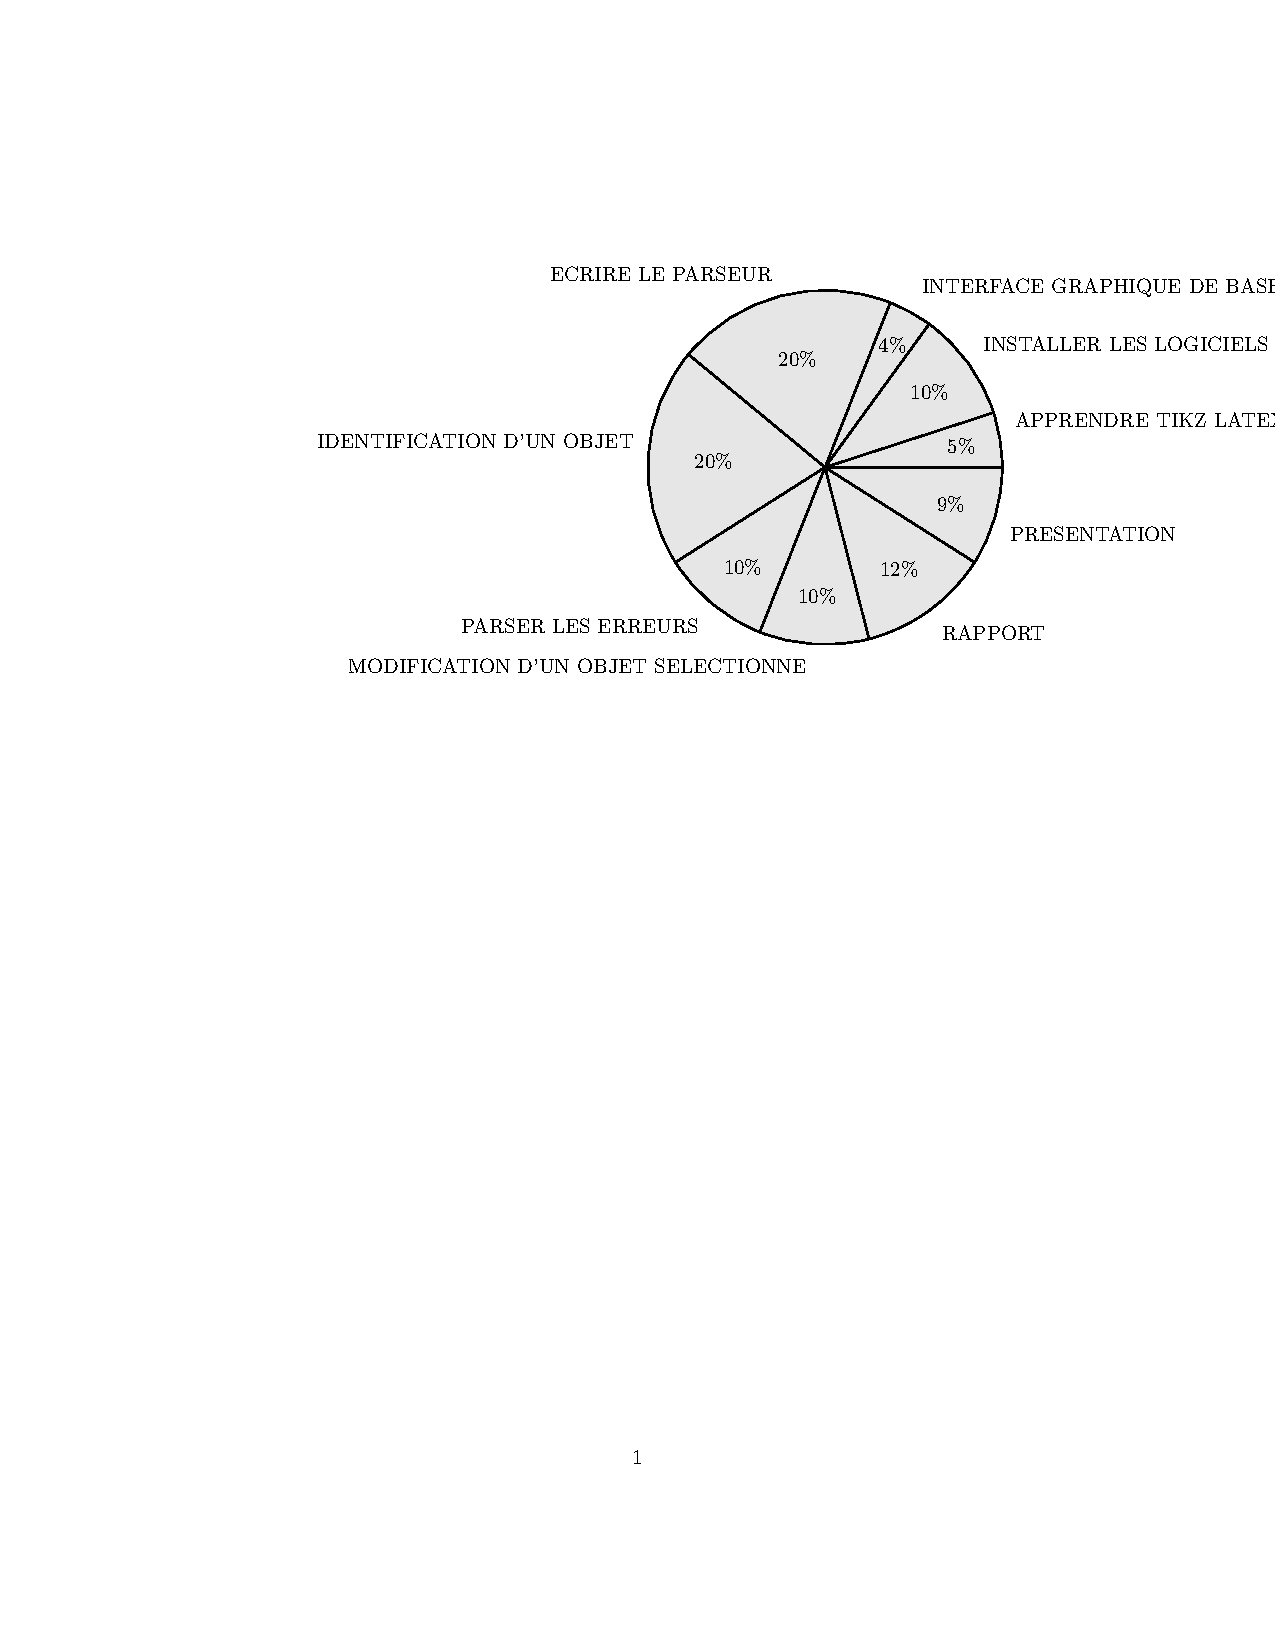
\includepdf{camembtex.pdf}
\section{Résultats}
  Nous allons à présent vous présenter en images les résultats de notre projet .
\newline
  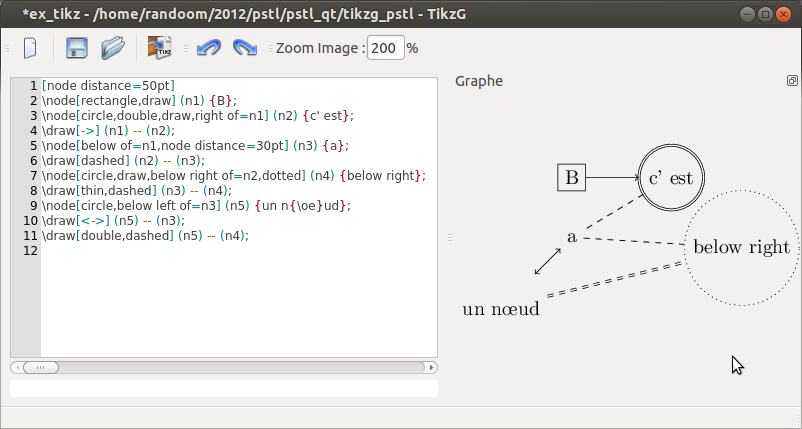
\includegraphics[width=15cm, height=10cm]{img/r_1.png} 
\newline
figure 1: génération du graphe à partir du code tikz édité
\\
\\
\\
\\
  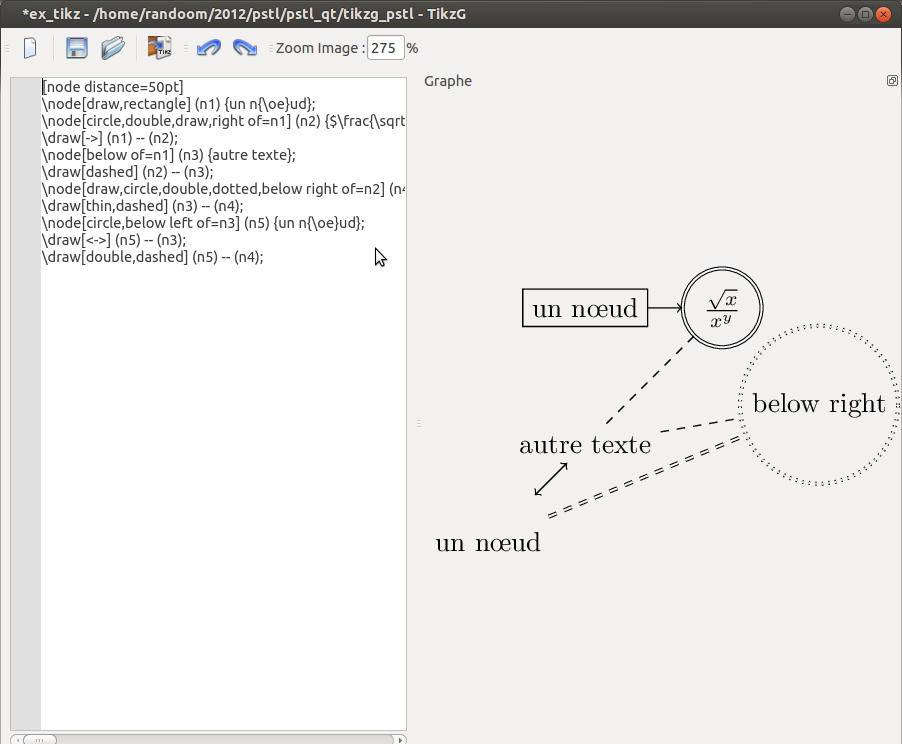
\includegraphics[width=15cm, height=10cm]{img/r_41.png} 
\\
figure 2: zoom et désactivation de la coloration syntaxique et des numéros de ligne dans la marge
\newline
\\
\\
\\
\\
  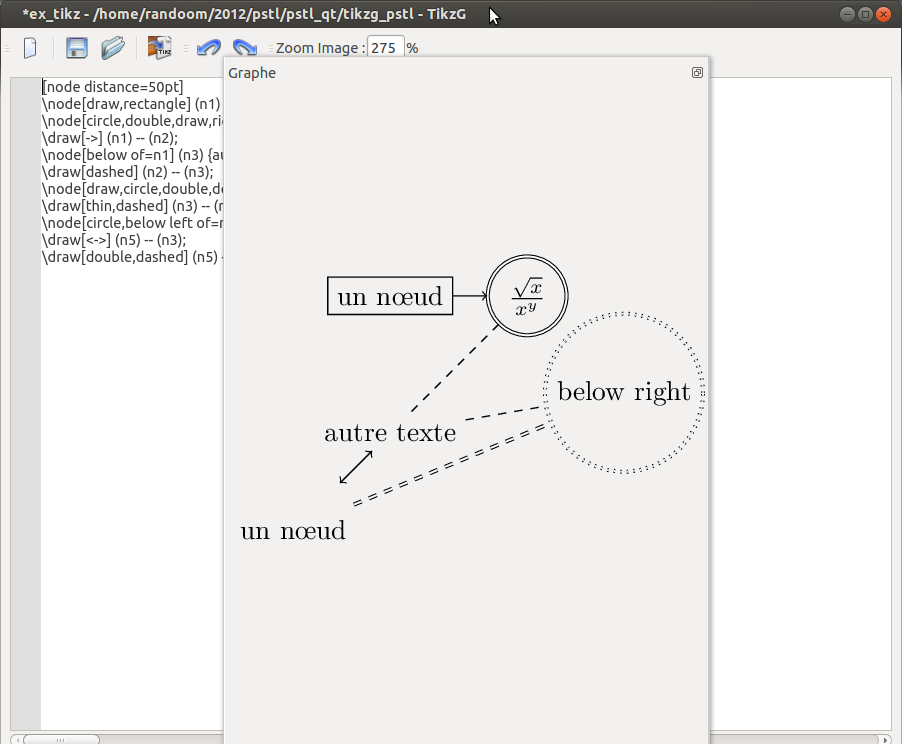
\includegraphics[width=15cm, height=10cm]{img/r_42.png} 
\\
figure 3: fenêtre du graphe flottante
\newline
\\
\\
\\
\\
  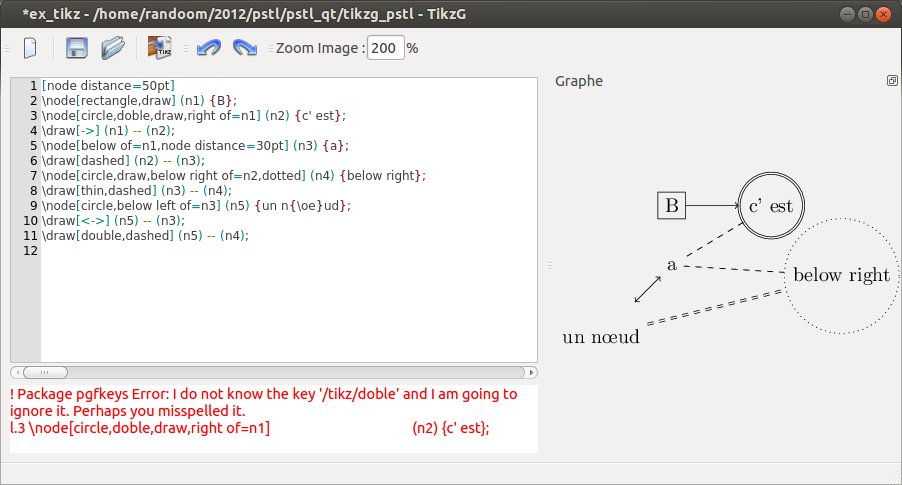
\includegraphics[width=15cm, height=10cm]{img/r_2.png} 
\\
figure 4: gestion d'erreurs
\\
\\
	Comme nous pouvons le constater sur la figure 1, le graphe est généré à partir du code Tikz écrit dans l'éditeur de texte. Cette génération est relancée automatique au bout d'une seconde d'inactivité après modification du code source. L'utilisateur pourra choisir de cacher les numéros de ligne ou de désactiver la coloration syntaxique en décochant les cases correspondantes dans la barre de menu ; il pourra aussi définir la valeur du zoom dans la barre d'outil ou zoomer avec la molette de la souris. En effet, sur la figure 1 on peut noter l'affichage des numéros de ligne, la coloration syntaxique du code et la valeur du zoom qui est de 200\%
alors que sur la figure 2 l'affichage des numéros de ligne est désactivée de même que la coloration syntaxique et la valeur du zoom vaut 275\% après un zoom avec la molette de la souris.

De plus, comme l'atteste les figures 3 et 4, les erreurs sont gérees et la fenêtre du graphe peut être détachée de l'interface et déplacée sans que cela ne modifie ses fonctionnalités.
\newline
  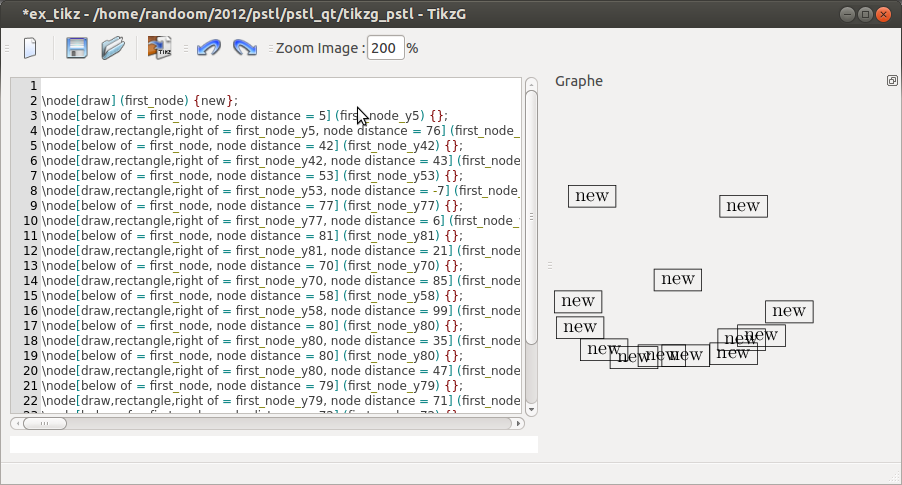
\includegraphics[width=15cm, height=10cm]{img/r_6.png} 
\\
  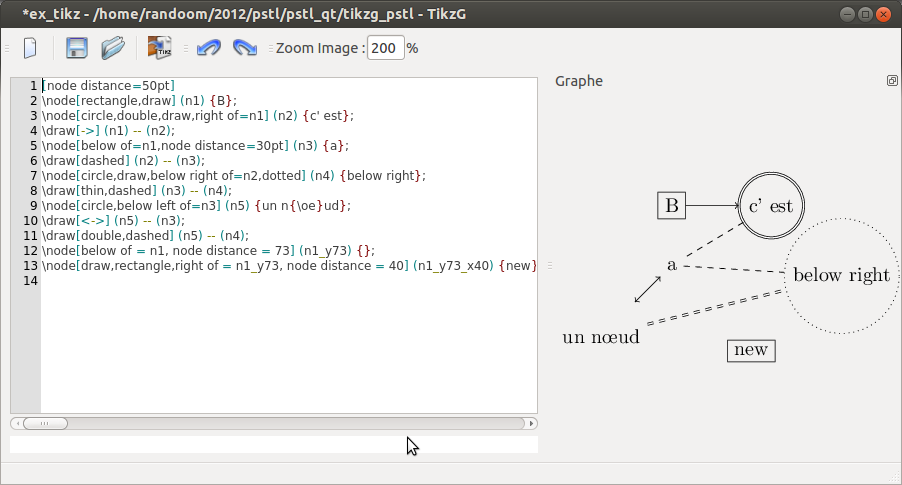
\includegraphics[width=15cm, height=10cm]{img/r_3.png}
\\ 
figures 5: création graphique d'un n{\oe}ud
\newline
  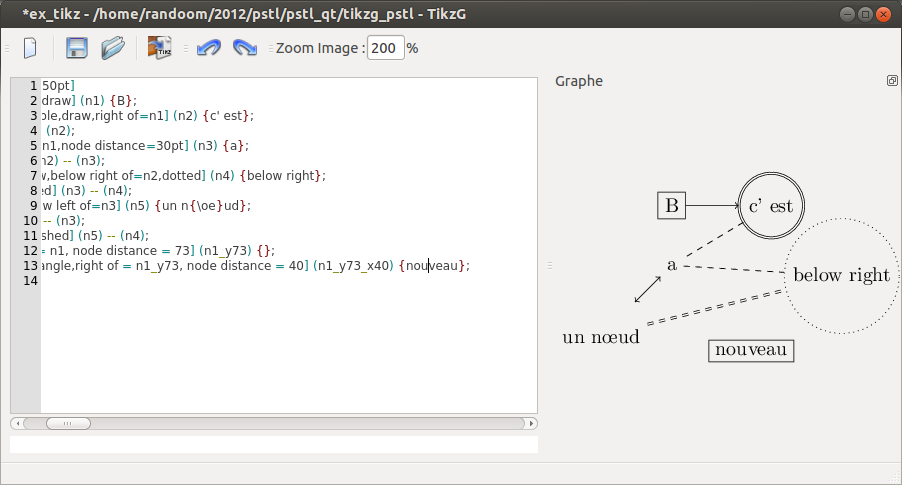
\includegraphics[width=15cm, height=10cm]{img/r_5.png} 
\\
figure 6: modification textuelle des propriétés d'un n{\oe}ud
\\
\\
Un clic droit sur l'interface graphique permet de créer un n{\oe}ud à cet endroit. L'utilisateur pourra par la suite modifier textuellement ou visuellement les propriétés de ce n{\oe}ud. Le code correspondant au noeud ainsi créé est automatique ajouter au code du graphe. 

Par exemple sur la figure 5, le n{\oe}ud contenant le texte "new" a été créé par un clic droit de la souris, et les  lignes 12 et 13 qui correspondent au code Tikz de la création de ce n{\oe}ud ont été ajouté à l'éditeur de texte. Après une modification sur le code du texte de ce n{\oe}ud(new qui devient nouveau), on observe sans surprise que le texte a aussi changé sur le graphe.
\newline
  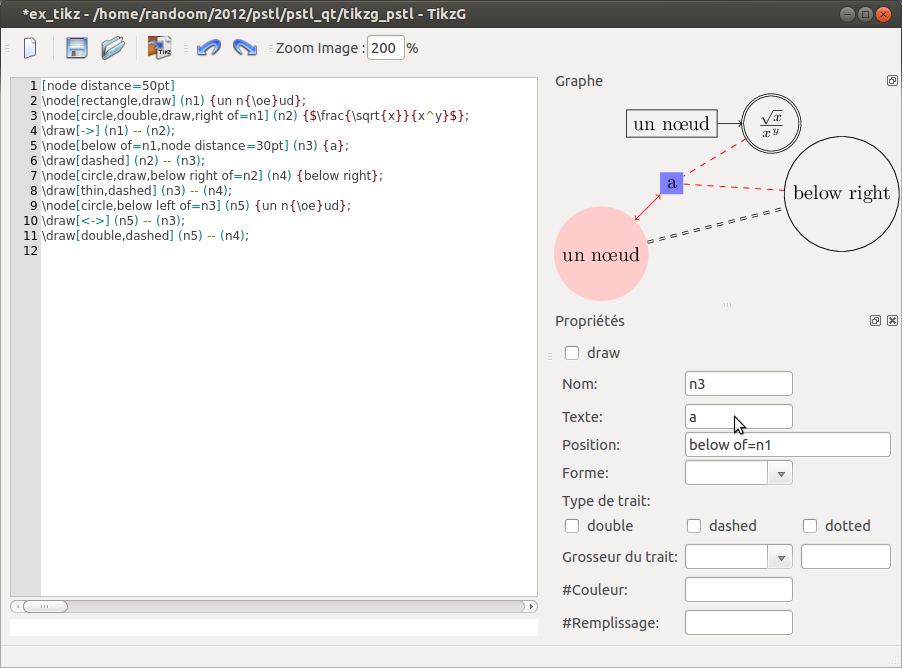
\includegraphics[width=15cm, height=10cm]{img/r_8.png} 
\\
  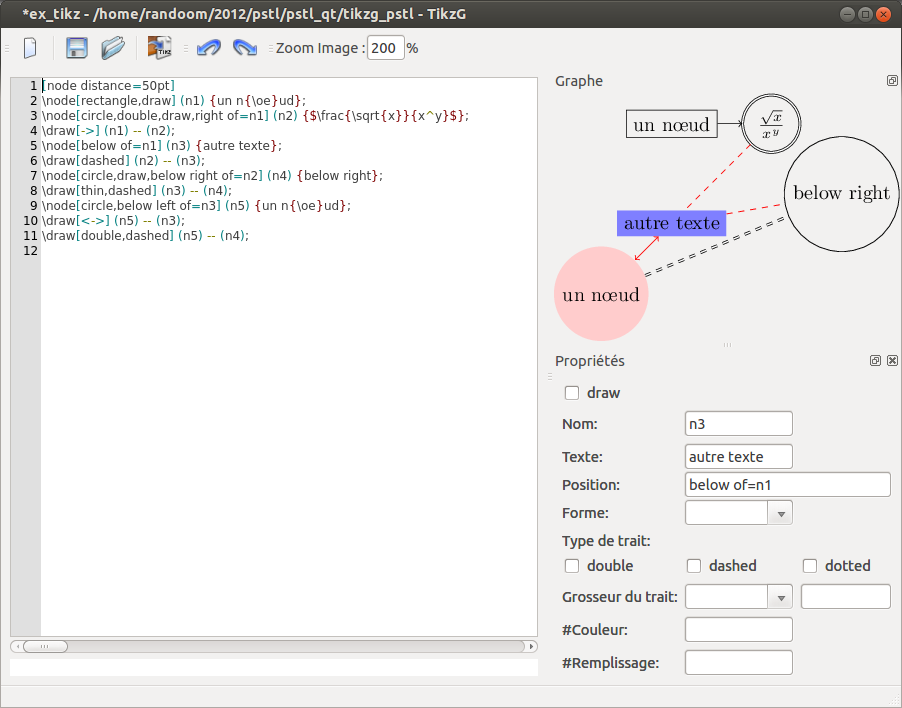
\includegraphics[width=15cm, height=10cm]{img/r_9.png}
\\ 
figures 7: modification graphique des propriétés d'un n{\oe}ud
\\
\\
Lorsqu'on clique sur un objet du graphe ses propriétés s'affichent. Prenons comme exemple les figures 7, on voit que lorsqu'on clique sur le noeud n3, il est coloré en bleu, ses noeuds relatifs en rose et les arêtes auxquelles il est rélié en rouge. A partir de sa fenêtre de propriétés on peut apporter des modifications au    n{\oe}ud ainsi sélectionné. Et comme on peut le remarquer sur ces figures, le texte "a" contenu dans ce noeud devient "autre texte" après une modification à partir de la fenêtre des propriétés.
\\
\\
\\
\\
\\
  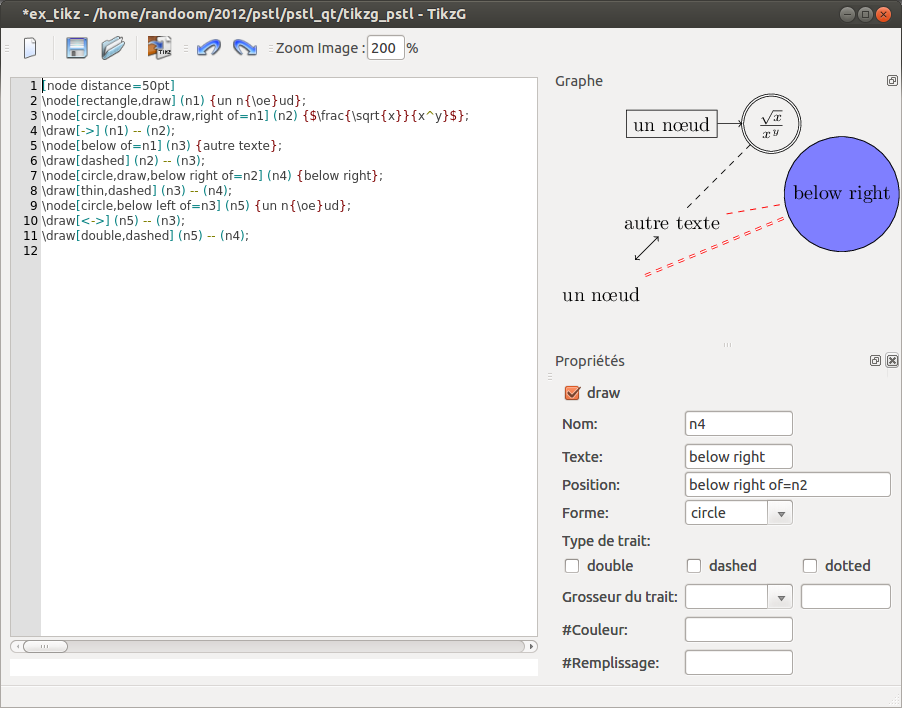
\includegraphics[width=15cm, height=10cm]{img/r_10.png}
\\ 
figure 10: sélection d'un n{\oe}ud du graphe

  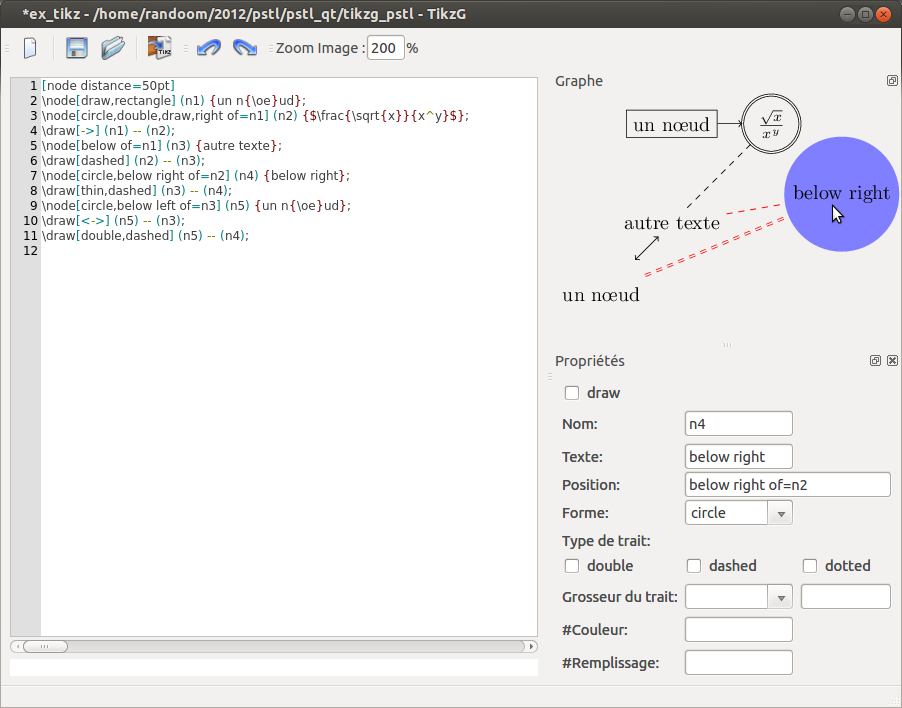
\includegraphics[width=15cm, height=10cm]{img/r_12.png}
\\ 
figure 11: modification d'un n{\oe}ud du graphe
\\
  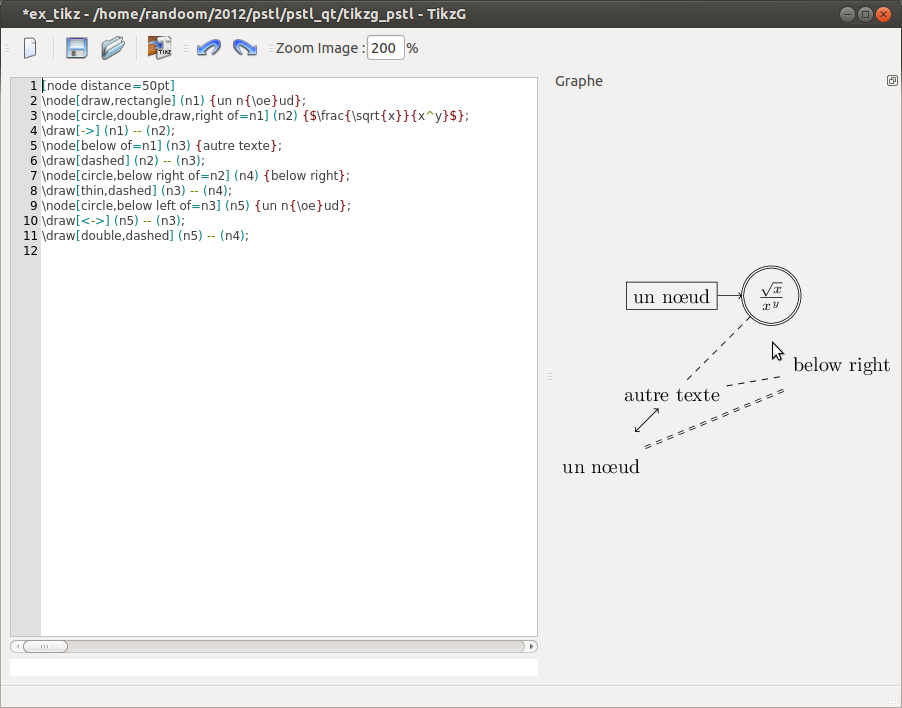
\includegraphics[width=15cm, height=9cm]{img/r_13.png}
\\ 
figure 12: après modification d'un n{\oe}ud du graphe
\\ \\
Les figures 10, 11 et 12 illustrent bien nos propos ci-dessus. On peut observer que sur la figure 10 dans la fenêtre Propriétés, la case draw qui correspond au dessin du n{\oe}ud est cochée après l'avoir décoché à la figure 11 on voit effectivement que, sur la figure  12, le noeud n'est plus dessiné et la propriété "draw" a disparu à la ligne 7 du code Tikz.
\\ \\ \\ \\ \\
  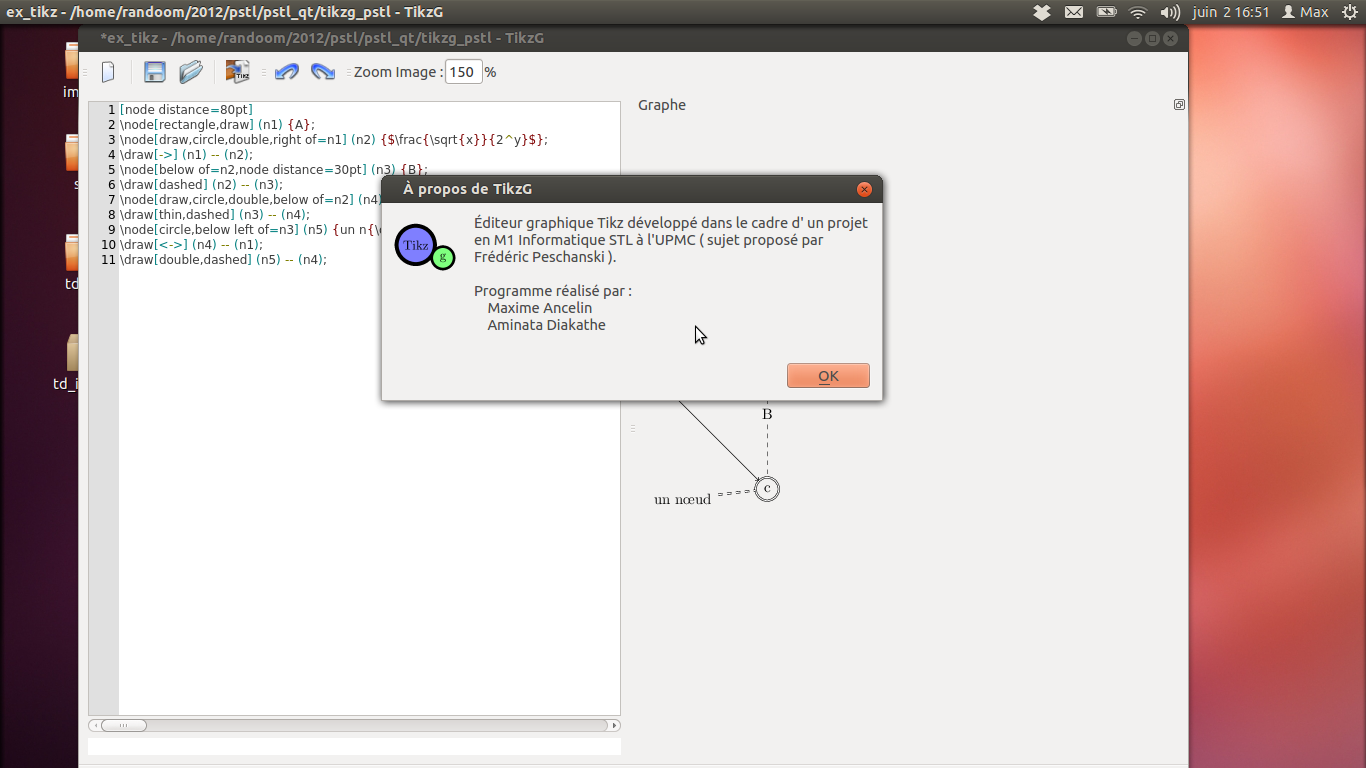
\includegraphics[width=15cm, height=9cm]{img/r7.png}
\\ 
figures 12: à propos
\chapter{Conclusion}
Nous avons créer une interface graphique permettant d'éditer du code Tikz, de visualiser l'image généré et de modifier visuellement les propriétés des n{\oe}uds dans le cadre de notre projet Science et Technologie de Logiciel. En effet, avec notre interface graphique l'utilisateur pourra désormais créer graphiquement des noeuds, modifier les propriétés des objets du graphe sélectionnés tout en récupérant le code Tikz correspondant à la création de ce graphe. Il pourra aussi charger directement un fichier Tikz dans l'éditeur afin de visualiser et/ou modifier le graphe. Le code Tikz édité pourra ainsi être sauvegardé de même que le fichier pdf généré par le code Latex englobant le code Tikz. 

Ce projet nous a permis d’appliquer les connaissances qui nous ont été inculquées au cours
de nos années de Licence et de Maîtrise Informatique à l’Université Pierre et Marie Curie. Nous avons été confrontés à de nombreux problèmes et dans la plupart des cas nous avons pu trouver une solution alternative afin de les résoudre.

Enfin ce projet aura été l’occasion de découvrir et d’utiliser des outils dont nous n’avions pas la
moindre idée de leurs existences.



\chapter{Perspectives}
Au vu des fonctionnalités de notre interface, nous pouvons conclure que les principaux objectifs du projet sont atteints. Toutefois, afin de faciliter la distribution de notre logiciel, nous aurions pu créer un paquet Debian et un exécutable Windows. De même pour une amélioration future de l'application, la gestion de la modification visuelle de la position d'un noeud pourra être réaliser. Cependant, le temps et la
complexité de ces tâches ont été les principaux facteurs qui nous ont rebuté. 

\chapter{Bibliographie}

Introduction à Perl \\
    \indent{Auteur(s) : Randal L. Schwartz , Tom Phoenix}\\
    \indent{Editeur : O'Reilly} \\ \\ \\

De l'art de programmer en Perl \\
    \indent{Auteur(s) : Damian Conway}\\
    \indent{Editeur : O'Reilly} \\ \\ \\

Perl Cookbook: \\
    \indent{Auteur(s) : Christiansen}\\ \\ \\

Tikz pour l'impatient (livre en français):\\
    \indent{http://math.et.info.free.fr/TikZ/bdd/TikZ-Impatient.pdf}\\ \\ \\

Introduction à Latex:\\
    \indent{http://mirrors.ctan.org/info/lshort/french/lshort-fr.pdf }



\chapter{Annexe}

\includepdf[pages = {1-9}]{manuel.pdf}
%n{\oe}ud

\end{document}


